% ============================================================================
% Sección: Configuración Experimental (Setup Mizuno-like, TEST=35A)
% Notas internas (no se renderizan):
%   - Se omite por completo cualquier referencia al Caso 35B (perfil invertido).
%   - Se conservan textualmente las ecuaciones de Vy y Vx provistas por el autor.
%   - Se documenta el sistema de unidades naturales racionalizadas (c=mu_0=eps_0=1)
%     y la equivalencia física del tiempo de simulación.
%   - Las variables de control de enstrofía (Omega_z, Omega_tot, f_Vz, Omega'_z)
%     se referencian al marco teórico previamente desarrollado, evitando duplicar
%     definiciones formales.
%   - La figura de inicialización se compone de DOS paneles efectivos:
%       (a) Campo vectorial de velocidad (streamlines + magnitud).
%       (b) Campo escalar de densidad rho.
%     Ambos paneles se renderizan en el primer snapshot diagnóstico (t=0001),
%     próximo al estado inicial t=0.
%   - Requiere el paquete subcaption en el preámbulo: \usepackage{subcaption}
% ============================================================================

\section{Configuración Experimental}
\label{sec:setup_experimental}

Para estudiar el impacto de la resistividad sobre la evolución lineal y no lineal de la Inestabilidad de Kelvin-Helmholtz (KHI), se llevaron a cabo simulaciones numéricas bidimensionales con el código \textit{Cueva}, el cual integra las ecuaciones de la Magnetohidrodinámica Relativista Resistiva (RRMHD) en la forma fuertemente conservativa expuesta en la Sección~\ref{sec:RRMHD_Conservativa}. La discretización espacial se realiza mediante un esquema de volúmenes finitos de alta resolución con reconstrucción \textit{Monotonicity-Preserving} de quinto orden (MP5), flujos numéricos HLL y limpieza hiperbólica de divergencias bajo el formalismo GLM (Sección~\ref{sec:Max-aumentado}). La integración temporal del sistema rígido inducido por los términos fuente resistivos se realiza con un esquema IMEX de Runge--Kutta. A continuación, se detallan las condiciones iniciales, el dominio computacional, el sistema de unidades adoptado y las variables de diagnóstico utilizadas.

\subsection{Condiciones Iniciales del Problema}
\label{subsec:condiciones_iniciales}

El escenario base corresponde a una configuración de cizalladura dual (Test 35A) directamente inspirada en el setup canónico de \parencite{mizuno-2013}, adaptado para aislar de forma controlada el desarrollo de los vórtices de KHI en el marco RRMHD bajo condiciones de contorno periódicas a lo largo de la dirección del flujo (Figura~\ref{fig:setup_inicial}).

El flujo de fondo se establece a lo largo del eje $y$, con dos interfaces de cizalladura suaves ubicadas simétricamente en $x = \pm 0.5$. El perfil de velocidad longitudinal está dado por:
\begin{equation}
    V_y(x) = \begin{cases} 
      +v_{sh}\, \tanh\!\left(\dfrac{x - 0.5}{a_{kh}}\right) & \text{si } x \geq 0 \\[4pt]
      -v_{sh}\, \tanh\!\left(\dfrac{x + 0.5}{a_{kh}}\right) & \text{si } x < 0 
   \end{cases}
   \label{eq:Vy_profile}
\end{equation}
donde $v_{sh} = 0.5\, c$ (factor de Lorentz relativo moderado $\Gamma_{\text{rel}} \simeq 1.29$) y $a_{kh} = 0.05$ define el ancho característico de la capa de cizalladura, garantizando que la escala dominante $k_{kh}^{-1}\!\gtrsim\!a_{kh}$ permita una resolución espectral adecuada del modo lineal inestable.

Para desencadenar selectivamente la inestabilidad mediante un único modo normal de longitud de onda compatible con el dominio periódico, se introduce una perturbación transversal localizada de la forma:
\begin{equation}
    V_x(x,y) = \begin{cases} 
      +V_0\, v_{sh}\, \sin(k_{kh}\, y)\, \exp\!\left[-\!\left(\dfrac{x - 0.5}{\alpha_{kh}}\right)^{\!2}\right] & \text{si } x \geq 0 \\[6pt]
      -V_0\, v_{sh}\, \sin(k_{kh}\, y)\, \exp\!\left[-\!\left(\dfrac{x + 0.5}{\alpha_{kh}}\right)^{\!2}\right] & \text{si } x < 0 
   \end{cases}
   \label{eq:Vx_pert}
\end{equation}
con amplitud modulada $V_0 = 1.0$, número de onda $k_{kh} = 2\pi/L_y$ (modo fundamental compatible con la periodicidad del dominio) y ancho gaussiano de confinamiento $\alpha_{kh} = 0.2$, lo cual restringe la inyección de energía cinética perturbativa al entorno inmediato de las capas de cizalladura. La componente $V_z$ se inicializa estrictamente nula, en consistencia con el carácter planar 2D de la simulación.

El perfil de densidad sigue la configuración canónica Mizuno-like: el flujo central (interior, $|x|<0.5$) presenta densidad baja, mientras que las regiones externas mantienen una densidad mayor. La transición se construye mediante una ventana suave a partir de funciones tangentes hiperbólicas:
\begin{equation}
\begin{aligned}
    \rho(x) &= \rho_{lo} + (\rho_{up} - \rho_{lo})\left[\,1 - W(x)\,\right],\\[2pt]
    W(x) &= \tfrac{1}{2}\!\left[1 + \tanh\!\left(\tfrac{x+0.5}{a_{kh}}\right)\right]\!\cdot\!\tfrac{1}{2}\!\left[1 - \tanh\!\left(\tfrac{x-0.5}{a_{kh}}\right)\right]
\end{aligned}
    \label{eq:rho_profile}
\end{equation}
con $\rho_{up} = 1.0$ y $\rho_{lo} = 0.1\,\rho_{up}$, lo que implica un contraste de densidad $\eta_\rho = \rho_{lo}/\rho_{up} = 0.1$ entre el flujo central y el ambiente envolvente. La presión térmica se asume inicialmente uniforme en todo el dominio con $P_0 = 1.0$, evitando así la inyección espuria de modos magnetoacústicos asociados a gradientes de presión iniciales.

En cuanto al campo magnético\sebnota{inconexo, necesita continuidad.}, se impone una configuración de fondo uniforme y desacoplada de la cizalladura, dominada por una componente fuera del plano y reforzada con una débil componente paralela a la interfaz:
\begin{equation}
    B_x = 0,\qquad B_y = B_0\,\sqrt{0.02},\qquad B_z = B_0\,\sqrt{2.0},
    \label{eq:B_field_init}
\end{equation}
con $B_0 = 1.0$. Este campo de fondo permanece fijo en los objetivos~1--3 (barrido en la conductividad $\sigma$); su intensidad y orientación se convierten en las variables de control en la campaña del objetivo~4 (Sección~\ref{subsec:campana_B}). Esta orientación garantiza que la tensión magnética longitudinal ($\mathbf{k}\cdot\mathbf{B}\propto B_y$) sea débil pero no nula, permitiendo el desarrollo de la KHI sin supresión inmediata, mientras que la componente $B_z$ dominante introduce una presión magnética fuera del plano significativa que regula la termodinámica del flujo. El campo eléctrico inicial se anula estrictamente, $E_x = E_y = E_z = 0$, lo que corresponde a un estado fuera del límite ideal $E^\mu = -\epsilon^{\mu\nu\alpha\beta} u_\nu B_\alpha v_\beta$; la ley de Ohm relativista (Sección~\ref{sec:Ohm_Relativista}) se encarga de relajar dinámicamente el sistema hacia su régimen consistente con la conductividad finita prescrita.

% ----------------------------------------------------------------------------
% Figura compuesta: condición inicial visualizada en el primer snapshot
% diagnóstico (t=0001 ~ estado inicial). Panel (a): campo vectorial de
% velocidad con líneas de corriente y magnitud |V| en mapa de color.
% Panel (b): campo escalar de densidad rho con contornos de nivel.
% NOTA: ajustar los nombres de archivo a los reales en el directorio /figuras/.
% ----------------------------------------------------------------------------






% Figura de condición inicial: dos paneles (velocidad y densidad) vía minipage.
\begin{figure}[h]
    \centering
    % --------------------------------------------------------------------
    % Panel (a): Campo vectorial de velocidad (streamlines + |V|)
    % --------------------------------------------------------------------
    \begin{minipage}{0.95\textwidth}
        \centering
        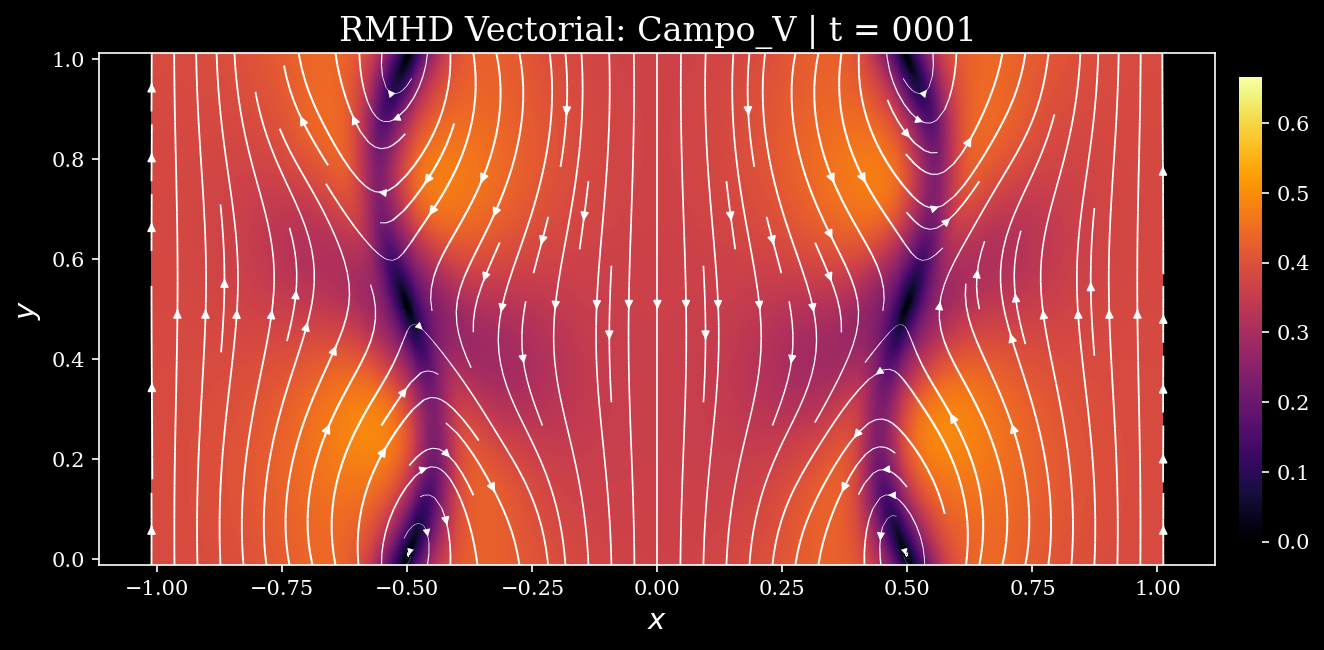
\includegraphics[width=\linewidth]{figuras/campo_V_inicial.png}
        % \includegraphics[width=\linewidth]{figuras/frame_0001_campoV.png}

        \vspace{0.3em}
        \small (a) Campo vectorial de velocidad: líneas de corriente superpuestas al mapa de color de la magnitud $|\mathbf{V}(x,y)|$. Se aprecian las dos capas de cizalladura simétricas localizadas en $x = \pm 0.5$ (regiones oscuras de baja magnitud), el cambio de signo de $V_y$ a través de cada interfaz, y la modulación senoidal transversal de período $L_y$ introducida por la perturbación de la Ec.~(\ref{eq:Vx_pert}), responsable de la semilla del modo inestable dominante.
    \end{minipage}

    \vspace{1.0em}

    % --------------------------------------------------------------------
    % Panel (b): Distribución escalar de densidad rho(x,y)
    % --------------------------------------------------------------------
    \begin{minipage}{0.95\textwidth}
        \centering
        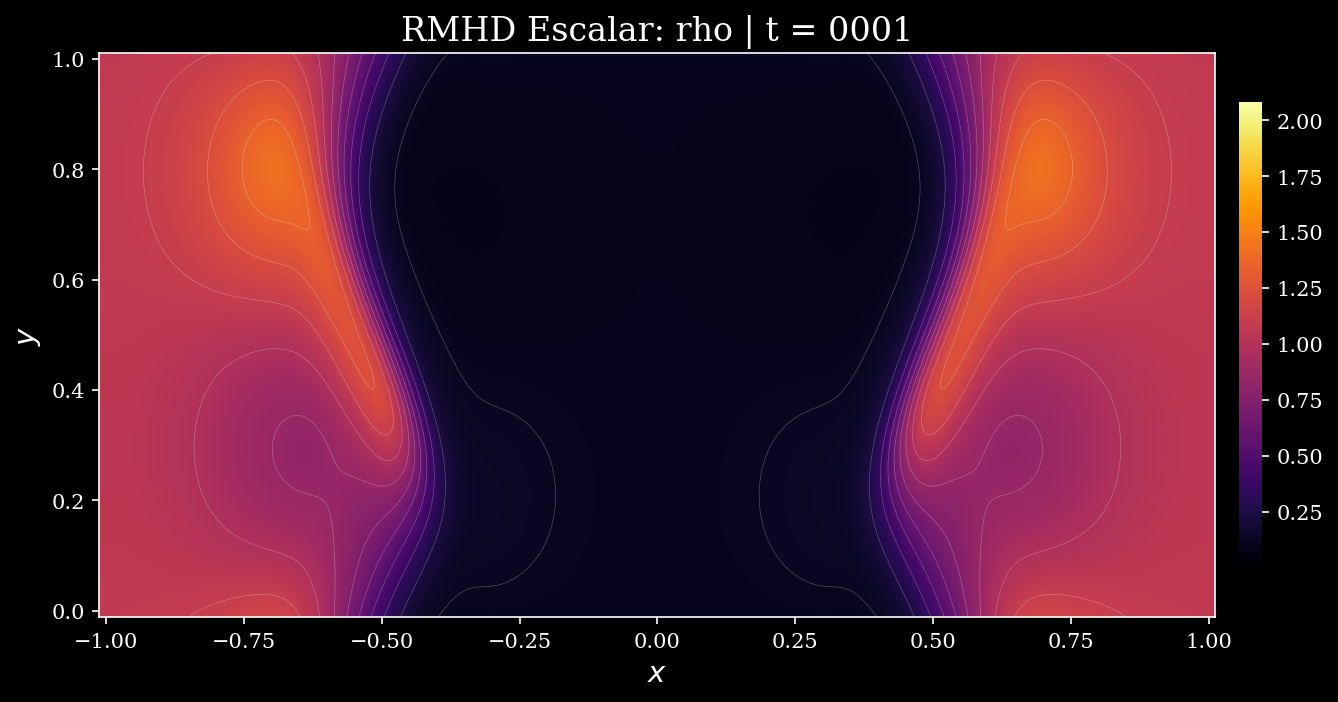
\includegraphics[width=\linewidth]{figuras/rho_inicial.png}
        % \includegraphics[width=\linewidth]{figuras/frame_0001_rho.png}

        \vspace{0.3em}
        \small (b) Distribución de densidad $\rho(x,y)$ con contornos isóbaros superpuestos. Se observa nítidamente la región interior de baja densidad ($\rho \simeq \rho_{lo}$, $|x| < 0.5$) embebida en el ambiente externo de alta densidad ($\rho \simeq \rho_{up}$, $|x| > 0.5$), consistente con la ventana hiperbólica prescrita por la Ec.~(\ref{eq:rho_profile}). Las modulaciones longitudinales tempranamente visibles en las interfaces reflejan la incipiente respuesta vortical del fluido a la perturbación inyectada.
    \end{minipage}

    \caption{Visualización del estado inicial del experimento KHI (Test~35A, primer snapshot diagnóstico $t \simeq 0$). Panel superior~(a): topología del campo de velocidad con sus dos capas de cizalladura simétricas y la perturbación senoidal de Kelvin--Helmholtz. Panel inferior~(b): perfil de densidad Mizuno-like, con flujo central diluido y ambiente externo denso. Estas dos distribuciones, junto con el campo magnético uniforme de fondo (Ec.~\ref{eq:B_field_init}), constituyen el estado base sobre el que se realiza el barrido paramétrico en la conductividad $\sigma$.}
    \label{fig:setup_inicial}
\end{figure}

\subsection{Dominio Computacional, Discretización y Sistema de Unidades}
\label{subsec:dominio_unidades}

El dominio de simulación se define como una caja cartesiana bidimensional que abarca $x \in [-1.0,\,1.0]$ y $y \in [-0.5,\,0.5]$, con dimensiones físicas $L_x = 2.0$ y $L_y = 1.0$ en unidades de código. La discretización se realiza sobre una malla uniforme y estructurada de $N_x \times N_y = 512 \times 256$ celdas, lo que produce un espaciamiento de $\Delta x = \Delta y \approx 3.906 \times 10^{-3}$ y garantiza una resolución de aproximadamente $a_{kh}/\Delta x \approx 12.8$ celdas a través de la capa de cizalladura, suficiente para resolver la fase lineal del modo dominante sin contaminación numérica significativa por difusividad de truncamiento.

Se emplean condiciones de contorno periódicas en la dirección $y$  y condiciones de frontera abiertas (flujo libre, derivadas normales nulas) en la dirección $x$\sebnota{Mirar bien en el código las condiciones de frontera.}\claudenota{Según el propio §\ref{subsec:dominio_unidades} y el código: periódicas en $y$ y abiertas (derivada normal nula / flujo libre) en $x$. Confirmar el flag exacto en \texttt{parameters.f95}; la descripción del texto es consistente.}, lo que minimiza las reflexiones espurias de ondas magnetoacústicas hacia el centro del dominio. El paso temporal se regula dinámicamente bajo la restricción Courant--Friedrichs--Lewy con $\text{CFL} = 0.1$, valor conservador requerido por la rigidez introducida por la corriente resistiva $\sigma E^\mu$ en el régimen de alta conductividad. La ecuación de estado adoptada es la del gas ideal politrópico con índice adiabático $\Gamma = 4/3$, consistente con un plasma ultrarrelativista dominado por presión de radiación.

\paragraph{Sistema de unidades y equivalencia temporal.} Las simulaciones se ejecutan en el sistema de unidades naturales racionalizadas de Heaviside--Lorentz adoptado a lo largo del marco teórico ($c = \mu_0 = \epsilon_0 = 1$). Bajo esta convención, todas las cantidades del código son adimensionales y se expresan en términos de una escala de longitud característica del problema $L_0$, fijada implícitamente por $L_y = 1$. La equivalencia con cualquier escenario físico se obtiene mediante el reescalado:
\begin{equation}
    t_{\text{fis}} = \frac{L_0}{c}\, t_{\text{cod}},\qquad
    x_{\text{fis}} = L_0\, x_{\text{cod}},\qquad
    \rho_{\text{fis}} = \rho_0\, \rho_{\text{cod}},\qquad
    B_{\text{fis}} = B_0^{\text{fis}}\, B_{\text{cod}},
    \label{eq:unidades_reescalado}
\end{equation}
donde $L_0$ y $\rho_0$ son escalas de referencia dimensionales y $B_0^{\text{fis}} = \sqrt{4\pi\rho_0 c^2}$ en unidades gaussianas. En consecuencia, la unidad de tiempo del código corresponde estrictamente al tiempo de cruce luminoso $\tau_c \equiv L_0 / c$ a través de la escala unitaria del dominio.

Las simulaciones de este estudio fueron ejecutadas para superar la marca de $t_{\text{cod}} > 5$ unidades de tiempo, lo cual equivale a $t_{\text{fis}} > 5\, L_0/c$. La elección de este horizonte temporal garantiza la cobertura completa de las tres fases dinámicas esperadas: (i) la fase lineal de crecimiento exponencial del modo perturbativo dominante; (ii) la fase de transición al régimen no lineal con formación de vórtices coherentes; y (iii) la fase de saturación con eventual cascada turbulenta secundaria y disipación resistiva. Como referencia astrofísica indicativa, si se identifica $L_0$ con escalas típicas de chorros AGN ($L_0 \sim 10^{15}\text{--}10^{17}\,\text{cm}$), $7\,\tau_c$ representa intervalos físicos de minutos a horas; en cambio, para fusiones de objetos compactos ($L_0 \sim 10^{6}\,\text{cm}$), $7\,\tau_c \sim 230\,\mu\text{s}$. La interpretación específica depende del régimen astrofísico al que se mapee el resultado adimensional.\sebnota{Dar un ejemplo concreto con escalas astrofísicas, deduciendo las dimensiones e incluso mostrando el radio de un vórtice generado en los \textit{hd plots}.} Los parámetros operativos consolidados se resumen en la Tabla~\ref{tab:setup_summary}.

\begin{table}[h]
\centering
\caption{Parámetros operativos consolidados del setup numérico (Test~35A, Mizuno-like).}
\label{tab:setup_summary}
\begin{tabular}{lll}
\hline
\textbf{Parámetro} & \textbf{Símbolo} & \textbf{Valor (unidades de código)} \\
\hline
Dominio en $x$              & $[x_{\min}, x_{\max}]$ & $[-1.0,\, 1.0]$ \\
Dominio en $y$              & $[y_{\min}, y_{\max}]$ & $[-0.5,\, 0.5]$ \\
Resolución de la malla      & $N_x \times N_y$        & $512 \times 256$ \\
Velocidad de cizalladura    & $v_{sh}$                & $0.5\, c$ \\
Ancho de la capa            & $a_{kh}$                & $0.05$ \\
Ancho gaussiano perturbativo& $\alpha_{kh}$           & $0.2$ \\
Amplitud perturbativa       & $V_0$                   & $1.0$ \\
Número de onda KHI          & $k_{kh}$                & $2\pi/L_y$ \\
Densidad de fondo (externa) & $\rho_{up}$             & $1.0$ \\
Densidad interna (central)  & $\rho_{lo}$             & $0.1\,\rho_{up}$ \\
Presión térmica             & $P_0$                   & $1.0$ \\
Magnitud magnética base     & $B_0$                   & $1.0$ \\
Componentes $(B_x,B_y,B_z)$ & ---                     & $(0,\, \sqrt{0.02},\, \sqrt{2.0})$ \\
Índice adiabático           & $\Gamma$                & $4/3$ \\
Número de Courant           & $\text{CFL}$            & $0.1$ \\
Tiempo final de integración & $t_{\text{end}}$        & $>5\,L_0/c$ \\
\hline
\end{tabular}
\end{table}

\subsection{Primera campaña: variación de la conductividad (objetivos 1--3)}
\label{subsec:barrido_sigma}

\primerparrafo El diseño experimental se articula en \emph{dos campañas numéricas complementarias y de igual peso}, que comparten el mismo montaje base y exploran dos ejes físicos distintos de la no idealidad: la \textbf{conductividad} (esta sección; objetivos 1--3) y el \textbf{campo magnético} ---intensidad y orientación--- (Sección~\ref{subsec:campana_B}; objetivo 4). La primera caracteriza el papel de la resistividad y la segunda el del campo; ambas tienen el mismo protagonismo en este trabajo y, en conjunto, completan la descripción del impacto de la física no ideal sobre la KHI.

Esta primera campaña cuantifica el impacto de la disipación óhmica sobre la dinámica de la KHI mediante un barrido paramétrico controlado en la conductividad eléctrica escalar $\sigma$, manteniendo invariantes las condiciones iniciales fluidas, termodinámicas y topológicas descritas en la Sección~\ref{subsec:condiciones_iniciales}. Esta estrategia aísla de forma rigurosa la contribución de la difusividad magnética $\eta = 1/\sigma$ sobre la tasa de crecimiento del modo lineal y la morfología no lineal de saturación.

Los valores seleccionados de $\sigma$ abarcan desde el régimen altamente difusivo (resistivo) hasta el límite cuasi-ideal donde se recupera el congelamiento topológico del flujo:
\begin{equation}
    \sigma \in \{100,\, 300,\, 500,\, \ldots,\, 10\,250,\, 10\,500\}
    \qquad (N = 44\ \text{valores}),
    \label{eq:sigma_sweep}
\end{equation}
que abarcan dos órdenes de magnitud en $\sigma \in [100,\, 10\,500]$; la lista
completa de los $44$ valores explorados se tabula en el capítulo de resultados
(Tabla~\ref{tab:canonica_sigma}). La transición entre regímenes se caracteriza dimensionalmente mediante el número de Lundquist local $S = L_0 V_A / \eta$, donde $V_A$ es la velocidad de Alfvén local evaluada con las cantidades iniciales. Para los valores de $\sigma$ aquí explorados, $S$ varía a lo largo de varios órdenes de magnitud, permitiendo identificar la conductividad crítica $\sigma_{\text{crit}}$ por encima de la cual la dinámica reproduce asintóticamente los resultados de la MHD ideal y por debajo de la cual la difusión resistiva domina sobre la advección magnética.

\subsection{Segunda campaña: variación del campo magnético (objetivo 4)}
\label{subsec:campana_B}

\primerparrafo La segunda campaña aborda el cuarto objetivo ---evaluar cómo la \emph{intensidad} y la \emph{orientación} del campo magnético externo modifican la estabilización o amplificación de la KHI--- variando $\mathbf{B}$ sobre el mismo montaje base (Sección~\ref{subsec:condiciones_iniciales}), con la conductividad \emph{fija} para aislar el efecto magnético del resistivo. Tiene el mismo peso analítico que la campaña de resistividad. La campaña se organiza en tres familias complementarias, todas con $|\mathbf B|=\sqrt{2.02}\,B_0$ en el caso de referencia ($B_0=1$).

\paragraph{Campaña A — Intensidad (orientación Mizuno fija).} Se conserva la orientación del setup base y se escala la magnitud,
\begin{equation}
B_x=0,\qquad B_y=B_0\sqrt{0.02},\qquad B_z=B_0\sqrt{2.0},\qquad B_0\in\{0.25,\,0.5,\,1.0,\,1.5,\,2.0\}.
\end{equation}
Al variar $B_0$ dos órdenes de magnitud, la presión magnética $P_{\rm mag}=B^2/2$, el parámetro de plasma $\beta=2P_0/B^2\approx0.99/B_0^2$ y la magnetización $\sigma_m\approx B^2/(\rho h)\approx0.404\,B_0^2$ (con $\rho h=5$) recorren regímenes desde dominado por presión ($\beta\gg1$) hasta dominado por campo ($\beta<1$); se espera que el aumento de $B_0$ refuerce la tensión magnética y estabilice la KHI (Cuadro~\ref{tab:campana_A}).

\begin{table}[H]\centering
\caption{Campaña A (intensidad): magnitud, $\beta$ y magnetización por caso (orientación Mizuno fija; $P_0=1$, $\rho h=5$).}
\label{tab:campana_A}
\begin{tabular}{lcccc}
\hline
Caso & $B_0$ & $B^2=2.02\,B_0^2$ & $\beta=2/B^2$ & $\sigma_m\approx B^2/5$ \\
\hline
A1 & $0.25$ & $0.126$ & $15.84$ & $0.025$ \\
A2 & $0.50$ & $0.505$ & $3.96$  & $0.101$ \\
A3 & $1.00$ & $2.020$ & $0.99$  & $0.404$ \\
A4 & $1.50$ & $4.545$ & $0.44$  & $0.909$ \\
A5 & $2.00$ & $8.080$ & $0.25$  & $1.616$ \\
\hline
\end{tabular}
\end{table}

\paragraph{Campaña B — Orientación en el plano $y$--$z$ ($|\mathbf B|$ fijo).} Se rota el campo en el plano transversal conservando su magnitud,
\begin{equation}
B_x=0,\qquad B_y=B_{\rm tot}\sin\theta,\qquad B_z=B_{\rm tot}\cos\theta,\qquad B_{\rm tot}=\sqrt{2.02},
\end{equation}
con $\theta\in\{0,\,5.7,\,15,\,30,\,45,\,60,\,90\}^\circ$. El caso Mizuno original corresponde a $\theta_{\rm Mizuno}=\arctan\!\sqrt{0.02/2.0}\approx5.7^\circ$; el extremo $\theta=0^\circ$ es campo guía puro ($\mathbf B=B_{\rm tot}\hat z$) y $\theta=90^\circ$ es campo enteramente en $\hat y$ (Cuadro~\ref{tab:campana_B}). Esta familia aísla si la pequeña componente transversal $B_y$ del setup Mizuno tiene un efecto dinámico apreciable.

\begin{table}[H]\centering
\caption{Campaña B (orientación en el plano $y$--$z$, $|\mathbf B|=\sqrt{2.02}$ fijo). El caso Mizuno es $\theta\approx5.7^\circ$.}
\label{tab:campana_B}
\begin{tabular}{lccc}
\hline
Caso & $\theta$ & $B_y/B_{\rm tot}=\sin\theta$ & $B_z/B_{\rm tot}=\cos\theta$ \\
\hline
B1 & $0^\circ$    & $0$     & $1$     \\
B2 & $5.7^\circ$  & $0.099$ & $0.995$ \\
B3 & $15^\circ$   & $0.259$ & $0.966$ \\
B4 & $30^\circ$   & $0.500$ & $0.866$ \\
B5 & $45^\circ$   & $0.707$ & $0.707$ \\
B6 & $60^\circ$   & $0.866$ & $0.500$ \\
B7 & $90^\circ$   & $1$     & $0$     \\
\hline
\end{tabular}
\end{table}

\paragraph{Campaña C — Componente paralela al flujo (plano $x$--$z$, $|\mathbf B|$ fijo).} Se introduce una componente a lo largo de la dirección del flujo,
\begin{equation}
B_y=0,\qquad B_x=B_{\rm tot}\sin\theta,\qquad B_z=B_{\rm tot}\cos\theta,\qquad \theta\in\{0,\,30,\,60,\,90\}^\circ.
\end{equation}
A diferencia de la Campaña~B, la rotación genera aquí una componente $B_x$ \emph{paralela} al flujo de cizalla, que puede estabilizar de forma más directa las perturbaciones mediante tensión magnética a lo largo de la dirección del corte (Cuadro~\ref{tab:campana_C}).

\begin{table}[H]\centering
\caption{Campaña C (componente paralela al flujo, plano $x$--$z$, $|\mathbf B|=\sqrt{2.02}$ fijo).}
\label{tab:campana_C}
\begin{tabular}{lccc}
\hline
Caso & $\theta$ & $B_x/B_{\rm tot}=\sin\theta$ & $B_z/B_{\rm tot}=\cos\theta$ \\
\hline
C1 & $0^\circ$  & $0$     & $1$     \\
C2 & $30^\circ$ & $0.500$ & $0.866$ \\
C3 & $60^\circ$ & $0.866$ & $0.500$ \\
C4 & $90^\circ$ & $1$     & $0$     \\
\hline
\end{tabular}
\end{table}

\paragraph{Conductividades y paso temporal.} Cada familia se ejecuta a conductividad fija. Aunque el diseño original de la campaña fijaba únicamente $\sigma=6000$ (para aislar el efecto magnético del resistivo), en este trabajo se analizan \emph{ambas} conductividades: $\sigma=6000$ (valor de referencia, donde la KHI ya se desarrolla de forma intensa) y $\sigma=10000$ (régimen casi ideal), con el fin de determinar si los efectos magnéticos persisten o se modifican al pasar del régimen de transición al cuasi-ideal.\sebnota{revisar la matriz final $\sigma\times$CFL realmente usada: los datos de llegada incluyen también $\sigma=4500,5500,6500,7000$ y versiones CFL $0.10/0.04/0.02$; definir cuáles entran en la monografía.} A alta conductividad y campo fuerte el sistema se vuelve numéricamente rígido (la recuperación de primitivas puede fallar al formarse láminas de corriente agudas); reducir el número de Courant de CFL$=0.04$ a CFL$=0.02$ estabiliza esas corridas, por lo que $\sigma=10000$ se integra a CFL$=0.02$ y $\sigma=6000$ a CFL$=0.04$.\sebnota{la comparación entre $\sigma$ queda entonces a CFL mixto; decidir si se homogeniza para el análisis final.}

\primerparrafo Sobre cada corrida de la campaña se monitorean los mismos diagnósticos de la Sección~\ref{subsec:diagnostico} ($\Omega_{zp}$, $\gamma_{\mathrm{KHI}}=s/2$, $\Omega^{\max}_{zp}$, $t_{\mathrm{peak}}$, $J_{\max}$, $\int\mathbf{E}\!\cdot\!\mathbf{J}\,dA$ y $f_{Vz}$), evaluados ahora como función de la intensidad $B_0$ y del ángulo $\theta$. El criterio operativo es que el campo \emph{estabiliza} si $\gamma_{\mathrm{KHI}}$ y $\Omega^{\max}_{zp}$ decrecen y $t_{\mathrm{peak}}$ aumenta, y \emph{amplifica} en el caso contrario.\sebnota{el análisis cuantitativo (\,$\gamma$ vs $B$, $\Omega^{\max}$ vs $\theta$, conversión magnética--cinética\,) se desarrolla en el Capítulo~\ref{ch:results_discussion}; resultados \emph{preliminares}, pendientes de revisión a fondo (no fiarse aún del informe de llegada).}

\subsection{Variables de Control y Diagnóstico}
\label{subsec:diagnostico}

Para extraer rigurosamente la tasa de crecimiento $\gamma_{\text{KHI}}$ y evaluar el impacto disipativo del barrido en $\sigma$ sobre la dinámica vortical, se requiere un conjunto de métricas globales que no se vean contaminadas por la cizalladura del flujo base ni por los gradientes inherentes a las condiciones iniciales. Como se estableció formalmente en la sección dedicada a la formulación geométrica de la vorticidad y enstrofía dentro del marco teórico (Sección~\ref{sec:Energia_Momento} \emph{et seq.}), se adoptan como observables principales las distintas manifestaciones eulerianas de la enstrofía planar previamente definidas.

En particular, se monitorea de manera sistemática a lo largo de la integración temporal:\sebnota{Mirar cuáles de estos diagnósticos sí se usan y cuáles no; además, seguro se usan otros, como campos y energías.}\claudenota{Del código: se usan $\Omega_z$, $\Omega_{\rm tot}$, $f_{Vz}$ y $\Omega'_{zp}$ (estos en cap.~6) y además $J_{\max}$, $\int\mathbf E\!\cdot\!\mathbf J$ y $E_{\rm mag}$ (§\ref{sec:globales}). Conviene listar también estos últimos aquí para que la sección de diagnósticos quede completa.}
\begin{itemize}
    \item \textbf{Enstrofía planar bidimensional:} $\Omega_z(t) = \int (\partial_x V_y - \partial_y V_x)^2\, dA$, que cuantifica la energía rotacional asociada a la componente fuera del plano del campo de vorticidad euleriano y constituye el indicador primario del crecimiento vortical en la geometría 2D del problema.
    \item \textbf{Enstrofía total tridimensional euleriana:} $\Omega_{\text{tot}}(t)$, que incorpora contribuciones de los gradientes transversales de $V_z$ y permite detectar la activación de modos fuera del plano por acoplamiento magnético, aun en una simulación nominalmente bidimensional.
    \item \textbf{Factor de anisotropía estructural:} $f_{Vz}(t) = (\Omega_{\text{tot}} - \Omega_z)/\Omega_{\text{tot}}$, cuya desviación respecto a cero señala el inicio de la ruptura de simetría planar inducida por la tensión magnética fuera del plano y el acoplamiento tridimensional emergente.
    \item \textbf{Enstrofía de perturbación:} $\Omega'_z(t) = \int (\omega'_z)^2\, dA$, definida sobre la vorticidad perturbada $\omega'_z = \omega_z - \langle \omega_z(t=0) \rangle_y$, la cual sustrae el fondo de cizalladura inicial y constituye la métrica fundamental para la extracción de la tasa de crecimiento lineal mediante regresión sobre $\ln \Omega'_z(t) = a + 2\gamma_{\text{KHI}}\, t$, donde $a$ es una constante de ajuste (no debe confundirse con el \emph{offset} $C$ del modelo sigmoide del capítulo de resultados).
\end{itemize}
La evaluación discreta de estos diagnósticos se realiza mediante diferencias finitas centradas de segundo orden sobre el campo de velocidad reconstruido en los centros de celda, con integración por regla del trapecio sobre todo el dominio físico $A = L_x \times L_y$. La combinación de estos cuatro observables proporciona una caracterización integral altamente sensible al régimen disipativo, permitiendo aislar de forma cuantitativa los efectos de la conductividad finita sobre las distintas fases dinámicas de la KHI.